%%%%%%%%%%%%%%%%%%%%%%%%%%%%%%%%%%%%%%%%%%%%%%%%%%%%%%%%%%%%%%%%%%%%%%%%%%%%%%%%%%%%%%%%%%%%%%%%%%%%%%%%%%%%%%%%%%%%%%%%%%%%%%%%%%%%%%%%%%%%
%%%%%%%%%%%%%%%%%%%%%%%%%%%%%%%%%%%%%%%%%%%%%%%%%%%%%%%%%%%%%%%%%%%%%%%%%%%%%%%%%%%%%%%%%%%%%%%%%%%%%%%%%%%%%%%%%%%%%%%%%%%%%%%%%%%%%%%%%%%%
% Dies ist ein Kommentar, er wird bei der pdf-Erzeugung ignoriert.


% Dies ist eine LaTex-Vorlage für den Gebrauch im Physikalischen Praktikum I und ist als Hilfestellung zu verstehen, falls keine LaTex-Kenntnisse vorhanden sind. Einige nötige und nützliche Pakete sind bereits eingebunden und die Kapitel (\section) angelegt. Die Kapitel beinhalten teilweise Beispiele wie die Darstellung von Grafiken/Tabellen oder mathematischen Formeln sowie Referenzen/Zitationen. Nach den nun folgenden Paketeinbindungen und Definitionen können die Namen der Verfasser, der Versuchsname usw. eingegeben werden. 


%%%%%%%%%%%%%%%%%%%%%%%%%%%%%%%%%%%%%%%%%%%%%%%%%%%%%%%%%%%%%%%%%%%%%%%%%%%%%%%%%%%%%%%%%%%%%%%%%%%%%%%%%%%%%%%%%%%%%%%%%%%%%%%%%%%%%%%%%%%%
%%%%%%%%%%%%%%%%%%%%%%%%%%%%%%%%%%%%%%%%%%%%%%%%%%%%%%%%%%%%%%%%%%%%%%%%%%%%%%%%%%%%%%%%%%%%%%%%%%%%%%%%%%%%%%%%%%%%%%%%%%%%%%%%%%%%%%%%%%%%
\documentclass[a4paper,12pt,bibtotocnumbered]{scrartcl}

\usepackage[utf8]{inputenc} %Codierung des LaTeX-Dokumentes. Auf Windows-Maschinen ist statt utf8 auch ANSIC als Codierung möglich, aber unnötig, da utf8 in jeder Hinsicht besser als ANSI ist. Bei Linux: latin1 als Codierung, auf MacOS X: applemac
\usepackage[T1]{fontenc}
\usepackage[ngerman]{babel} %Deutsche Zeichen- und Umbruchsetzung
\usepackage{amsmath, amssymb,amsfonts} %AMS-TeX-Pakete. Nötig für die Definition der Mathematik-Umgebung
\usepackage{graphicx} %Nötig, um Grafiken einbinden zu können
\usepackage[bookmarks,colorlinks=true]{hyperref} %Mittels hyperref lassen sich hyperlinks innerhalb des PDF-Dokumentes benutzen. Beispiel: Mausklick im Inhaltsverzeichnis auf ein Kapitel führt zum automatischen Sprung in dieses Kapitel
\usepackage{geometry}
\usepackage{float}
%Ein Paket, mit dem sich ohne Probleme mehrseitige PDF-Dokumente ohne \includegraphics-Rumgemache einbinden lassen. Befehl: \includepdf[pages=a-b]{PDFfile.pdf}. Einzelne Seiten, oder auch alle Seiten (Option pages=-) können angewählt werden
%Wenn keine Option angegeben wird, gilt pages=1!
\usepackage[final]{pdfpages}
\usepackage{framed, color} %Framed: Paket, mittels dessen ein Rahmen um einen Bereich definiert werden kann. Color: Lässt Farbdarstellung in Schrift, Hintergrund etc. zu
\usepackage{scrlayer-scrpage} %Header für die KOMA-script -Klasse
\usepackage{siunitx} %Ein schönes Paket, um Einheiten und physikalische Größen richtig zu setzen. Z.B.  \SI{2}{\kilo\gram\per\meter\squared}
\usepackage[square,numbers]{natbib}
\usepackage{subfigure} %Mehrere Bilder in einer Figure-Umgebung
\usepackage{lipsum}  
\usepackage{setspace}
\usepackage{booktabs}
\usepackage{csquotes}
\MakeOuterQuote{"}


%siunitx-Konfiguration. Damit werden die richtigen Font-Einstellungen erkannt (also beispielsweise fett, kursiv etc.) und damit  ebenfalls die deutsche Zeichensetzung, insbesondere Trennungszeichen, benutzt werden. 
%Ebenso wird bei SIrange das "`to"' in "`bis"' umgewandelt, bei SIlist das "`and"' in "`und"'
\sisetup{detect-weight=true, detect-family=true,locale=DE,range-phrase={\,bis\,},list-final-separator ={\,\linebreak[0] \text{und}\,},separate-uncertainty=true,per-mode = symbol-or-fraction}
%\SI[per-mode = fraction]{1}{\meter\per\second} erzwingt auch im Fließtext die Bruchdarstellung.
\DeclareSIUnit\curie{Ci}%Zusätzliche Einheit definieren

%Hyperlinks-Setup
\hypersetup{
	colorlinks,
	linktoc=all,
	citecolor=black,
	filecolor=black,
	linkcolor=black,
	urlcolor=black
}

\numberwithin{equation}{section} % Die Nummerierung von Gleichungen bekommt die jeweilige Section-Nummer als Präfix

\setlength{\parindent}{0 mm} %Einrücktiefe von neuen Absätzen
\setlength{\parskip}{2 mm} %Abstand von Absätzen



\pagestyle{scrheadings}%Kopf und Fußzeilen
\ohead{\textbf{\VERSUCHSNR}} %Header oben links auf linker Seite (ungerade Seitenzahl) und oben rechts auf rechter Seite (gerade Seitenzahl), beinhaltet gruppennummer und Versuchskürzel. Im Fall eine einseitigen Dokuments: Header oben rechts
\ihead{113469b Praktikum 3D-Druck} %Header oben rechts auf linker Seite und oben links auf rechter Seite. Beinhaltet die Namen der Verfasser. Im Fall eine einseitigen Dokuments: Header oben links!
\ofoot{\thepage} %Footer unten links auf linker und unten rechts auf rechter Seite, enthält die jeweilige Seitenzahl. Im Fall eines einseitigen Elements: Footer unten rechts!
\cfoot{\empty} %Mittig unten im Footer soll nichts eingetragen werden 
\ifoot{\VerfasserEINS} %Footer unten rechts auf linker und unten links auf rechter Seite. Hier ebenfalls leer.


%%%%%%%%%%%%%%%%%%%%%%%%%%%%%%%%%%%%%%%%%%%%%%%%%%%%%%%%%%%%%%%%%%%%%%%%%%%%%%%%%%%%%%%%%%%%%%%%%%%%%%%%%%%%%%%%%%%%%%%%%%%%%%%%%%%%%%%%%%%%

% Hier können die individuellen Anpassungen vorgenommen werden, die sich auf das Titelblatt und die Kopfzeilen auswirken.

\newcommand{\VERSUCHSDATUM}{23.03.2022}
\newcommand{\PROTOKOLLDATUM}{\today}

\newcommand{\VerfasserEINS}{Hannes Frey}
\newcommand{\MatNoEINS}{39311}
\newcommand{\StudiengangEINS}{MI7}
\newcommand{\SemesterEINS}{6. Semester}
\newcommand{\MailEINS}{hf018@hdm-stuttgar.de}

\newcommand{\VerfasserZWEI}{Verfasser 2}
\newcommand{\MatNoZWEI}{Matrikelnummer 2}
\newcommand{\StudiengangZWEI}{Technologiemanagement}

\newcommand{\BETREUER}{Karl Schaschek}
\newcommand{\WORTZAHL}{2220}
\newcommand{\GRUPPENNR}{Z-999}

\newcommand{\VERSUCHSNR}{Übung 01}
\newcommand{\VERSUCHSNAME}{Justage des Abstandes Düse - Druckbett}

%%%%%%%%%%%%%%%%%%%%%%%%%%%%%%%%%%%%%%%%%%%%%%%%%%%%%%%%%%%%%%%%%%%%%%%%%%%%%%%%%%%%%%%%%%%%%%%%%%%%%%%%%%%%%%%%%%%%%%%%%%%%%%%%%%%%%%%%%%%%
% Hier beginnt die Titelseite

\begin{document}
\thispagestyle{empty}


\begin{titlepage}

\begin{center}
\Huge{\textbf{\VERSUCHSNR\ – \VERSUCHSNAME}}\\% \Huge \huge \Large \normalsize \Small usw. bestimmt die Schriftgröße.
\vspace{10mm}% Abstand
\Large{Protokoll zum Versuch des 3D-Druck Praktikums 113469  % von \\ \textbf{\VerfasserEINS\;}
}\\
\vspace{10mm} 
\Large{Hochschule der Medien Stuttgart}\\
\end{center}
\vspace{1cm}
\begin{center}
\begin{tabular}{ll}
\large{Verfasser:}		& \large{\VerfasserEINS\;(\StudiengangEINS, \SemesterEINS),} \\ 
						& \large{\MailEINS}, \\
 						& \large{\MatNoEINS} \\
% 						\vspace{0cm}\\
%						& \large{\VerfasserZWEI\;(\StudiengangZWEI),} \\
%						& \large{\MatNoZWEI} \\
						\vspace{0cm}\\
%\large{Gruppennummer:}	& \large{\GRUPPENNR} \\
\vspace{0cm}\\
\large{Versuchsdatum:}	& \large{\VERSUCHSDATUM} \\
\vspace{0cm}\\
\large{Betreuer:}		& \large{\BETREUER} \\
\vspace{0cm}\\
\large{Wortzahl:}		& \large{\WORTZAHL}
\end{tabular}
\end{center}
\vspace{65mm}

\begin{center}
Stuttgart, den \PROTOKOLLDATUM
\end{center}

\end{titlepage}


\thispagestyle{empty}
%%%%%%%%%%%%%%%%%%%%%%%%%%%%%%%%%%%%%%%%%%%%%%%%%%%%%%%%%%%%%%%%%%%%%%%%%%%%%%%%%%%%%%%%%%%%%%%%%%%%%%%%%%%%%%%%%%%%%%%%%%%%%%%%%%%%%%%%%%%%%%%%
%Mittels des untenstehenden einfachen Befehls wird ein Inhaltsverzeichnis angelegt. LaTeX erstellt das Inhaltsverzeichnis völlig automatisch anhand der Überschriften für Kapitel, Unterkapitel etc. Das Dokument muss
%unter Umständen zweimal neu gesetzt werden, damit Änderungen in den Überschriften auch im Inhaltsverzeichnis auftauchen!
%%%%%%%%%%%%%%%%%%%%%%%%%%%%%%%%%%%%%%%%%%%%%%%%%%%%%%%%%%%%%%%%%%%%%%%%%%%%%%%%%%%%%%%%%%%%%%%%%%%%%%%%%%%%%%%%%%%%%%%%%%%%%%%%%%%%%%%%%%%%%%%%
\tableofcontents 
%%%%%%%%%%%%%%%%%%%%%%%%%%%%%%%%%%%%%%%%%%%%%%%%%%%%%%%%%%%%%%%%%%%%%%%%%%%%%%%%%%%%%%%%%%%%%%%%%%%%%%%%%%%%%%%%%%%%%%%%%%%%%%%%%%%%%%%%%%%%%%%%
\clearpage %Neue Seite, davor werden alle noch ausstehenden Grafiken/Tabellen platziert.


\renewcommand{\thepage}{\arabic{page}}
\setcounter{page}{1}


%%%%%%%%%%%%%%%%%%%%%%%%%%%%%%%%%%%%%%%%%%%%%%%%%%%%%%%%%%%%%%%%%%%%%%%%%%%%%%%%%%%%%%%%%%%%%%%%%%%%%%%%%%%%%%%%%%%%%%%%%%%%%%%%%%%%%%%%%%%%
%%%%%%%%%%%%%%%%%%%%%%%%%%%%%%%%%%%%%%%%%%%%%%%%%%%%%%%%%%%%%%%%%%%%%%%%%%%%%%%%%%%%%%%%%%%%%%%%%%%%%%%%%%%%%%%%%%%%%%%%%%%%%%%%%%%%%%%%%%%%
%%%%%%%%%%%%%%%%%%%%%%%%%%%%%%%%%%%%%%%%%%%%%%%%%%%%%%%%%%%%%%%%%%%%%%%%%%%%%%%%%%%%%%%%%%%%%%%%%%%%%%%%%%%%%%%%%%%%%%%%%%%%%%%%%%%%%%%%%%%%

% Abbildungsverzeichnis
\listoffigures
\addcontentsline{toc}{section}{Abbildungsverzeichnis}

% Tabellenverzeichnis
\listoftables
\addcontentsline{toc}{section}{Tabellenverzeichnis}

\newpage
\onehalfspacing 

% Die erste eckige Klammer ist optional, die darin angegebene Bezeichnung steht im Inhaltsverzeichnis anstelle des hinteren (längeren) Namens.
\section[Einführung]{Einführung und Versuchsziel}

Dieser Versuch soll dazu dienen erste Schritte im Umgang mit einem FFM-Drucker zu erlernen, und sich dem darunterliegenden Workflow für folgende Versuche bewusst zu werden. Dazu wird in einem ersten Schritt ein stl-Modell eines simplen Quaders mit der Software PrusaSlicer für den 3D-Druck vorbereitet und per SD-Karte an den Drucker übertragen. Anschließend wird am Drucker der Druck gestartet und beobachtet, wie die erste Schicht Plastik aufgetragen wird. Um Folgen einer schlecht, beziehungsweise falsch eingestellten Drucknivellierung zu begreifen, beginnt man nach einiger Zeit die Einstellung "z-adjust" verändert, was das Offset der Höhe des Druckkopfes beeinflusst. 

\section[Verwendete Geräte, Materialien und Hilfsmittel]{Verwendete Geräte, Materialien und Hilfsmittel}

Zur Versuchsdurchführung wurde ein 3D Drucker der Marke Prusa, Modell i3 MK3S+ mit Filament des Typs PLA verwendet. Der gedruckte Prototyp musste mit einem Plastikspachtel von der Druckfläche entfernt werden.

Zur Protokollerstellung kam \LaTeX\;zum Einsatz, Screenshots des PrusaSlicers konnten mit der Windows eigenen Lösung erstellt werden. Bilder des gedruckten Objekts wurden mit einem Smartphone Marke Google erstellt, ein 2D-Scan mit einem Brother MFC-9332CDW Drucker.

\section[Versuchsdurchführung]{Versuchsdurchführung}

Zu Beginn wurde das Programm PrusaSlicer gestartet und das erscheinende "First-Steps" Modal abgearbeitet. Dabei wurden Einstellungen vorgenommen, wobei viele bereits durch die Auswahl des zu verwendenden Druckers vordefiniert wurden. Zudem wurde die Präferenz gesetzt "*.3mf" und ".stl" Dateien in PrusaSlicer zu öffnen um in Zukunft diese komfortabler öffnen zu können.
Im Anschluss wurde das vorgegebene stl-Model mit dem Programm für den 3D-Drucker vorbereitet, indem die Datei öber das Kontextmenü des Programms geladen wurde und man im oberen rechten Bereich des Programms die Qualitätseinstellungen (siehe Abb.\ref*{quality_settings}) für den Druck bestimmt, um daraufhin das Modell über den Button unten rechts zu "slicen" (Abb. \ref*{slice_now})


\begin{figure}[htbp]
\centerline{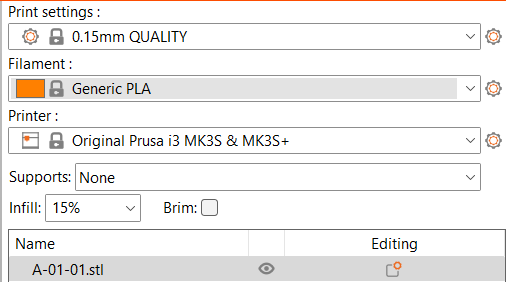
\includegraphics[width=200px]{./images/print_settings.png}}
\caption{PrusaSlicer - Qualitätsteinstellungen für das Slicen}
\label{quality_settings}
\end{figure}

\begin{figure}[htbp]
\centerline{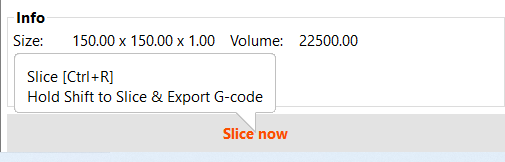
\includegraphics[width=200px]{./images/slice_now.png}}
\caption{PrusaSlicer - Button Slice Now}
\label{slice_now}
\end{figure}

Das so vorbereitete Modell kann dann auf eine SD-Karte gespeichert werden (Abb. \ref*{export}) und diese am Drucker eingesteckt werden um die Datei dort zu öffnen und in folgenden Schritten zu drucken.

\begin{figure}[htbp]
\centerline{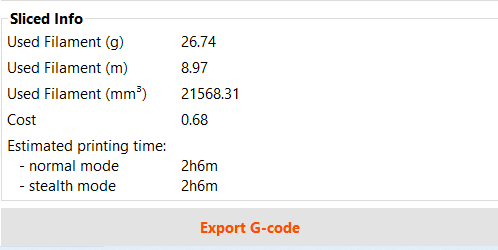
\includegraphics[width=200px]{./images/export.png}}
\caption{PrusaSlicer - Export G-code für den Druck}
\label{export}
\end{figure}

Anstatt direkt mit dem Drucken zu starten, wurde zunächst die Bedienoberfläche des Druckers untersucht um sich damit vertraut zu machen. Daraufhin konnte der Druck gestartet werden und nach kurzem warten darauf, dass der Drucker die zuvor eingestellten Drucktemperaturen erreicht hat, beginnt der Druck und das Verändern der z-Achsen adjustierung konnte vorgenommen werden. Hierfür konnten während des Drucks die Einstellung "z-live-adjust" am Bedienfeld des Druckers verwendet werden. Um objektive Aussagen zu treffen wurde der Druckkopf jeweils um 0.05mm in der Höhe verstellt, abhänging vom bisher eingestellten Ausgangspunkt $z_0$. Da nach bereits drei Höhenveränderungen je Richtung deutliche Ergebnisse zu sehen waren, wurden die Messungen damit beendet und die in Tabelle \ref*{z_adjust} zu sehenden z-Abstände entstanden.

\bgroup
\def\arraystretch{1.6}%
\begin{table}[]
\caption{Verwendete z-adjust Werte}
\centering
\begin{tabular}{|c|c|}
\hline
	 & Höhe (z-adjust) {[}mm{]} \\ \hline
z\_0 & -2,295                   \\ \hline
z\_1 & -2,345                   \\ \hline
z\_2 & -2,395                   \\ \hline
z\_3 & -2,445                   \\ \hline
z\_4 & -2,245                   \\ \hline
z\_5 & -2,195                   \\ \hline
z\_6 & -2,145                   \\ \hline
\end{tabular}
\label{z_adjust}
\end{table}
\egroup

\section[Auswertung und Analyse]{Auswertung und Analyse}

Die Bedienung des Programms PrusaSlicer, sowie die Oberfläche des Druckers waren sehr intuitiv nutzbar und es Bedarf keiner weiteren Analyse.


\begin{figure}[htbp]
\centerline{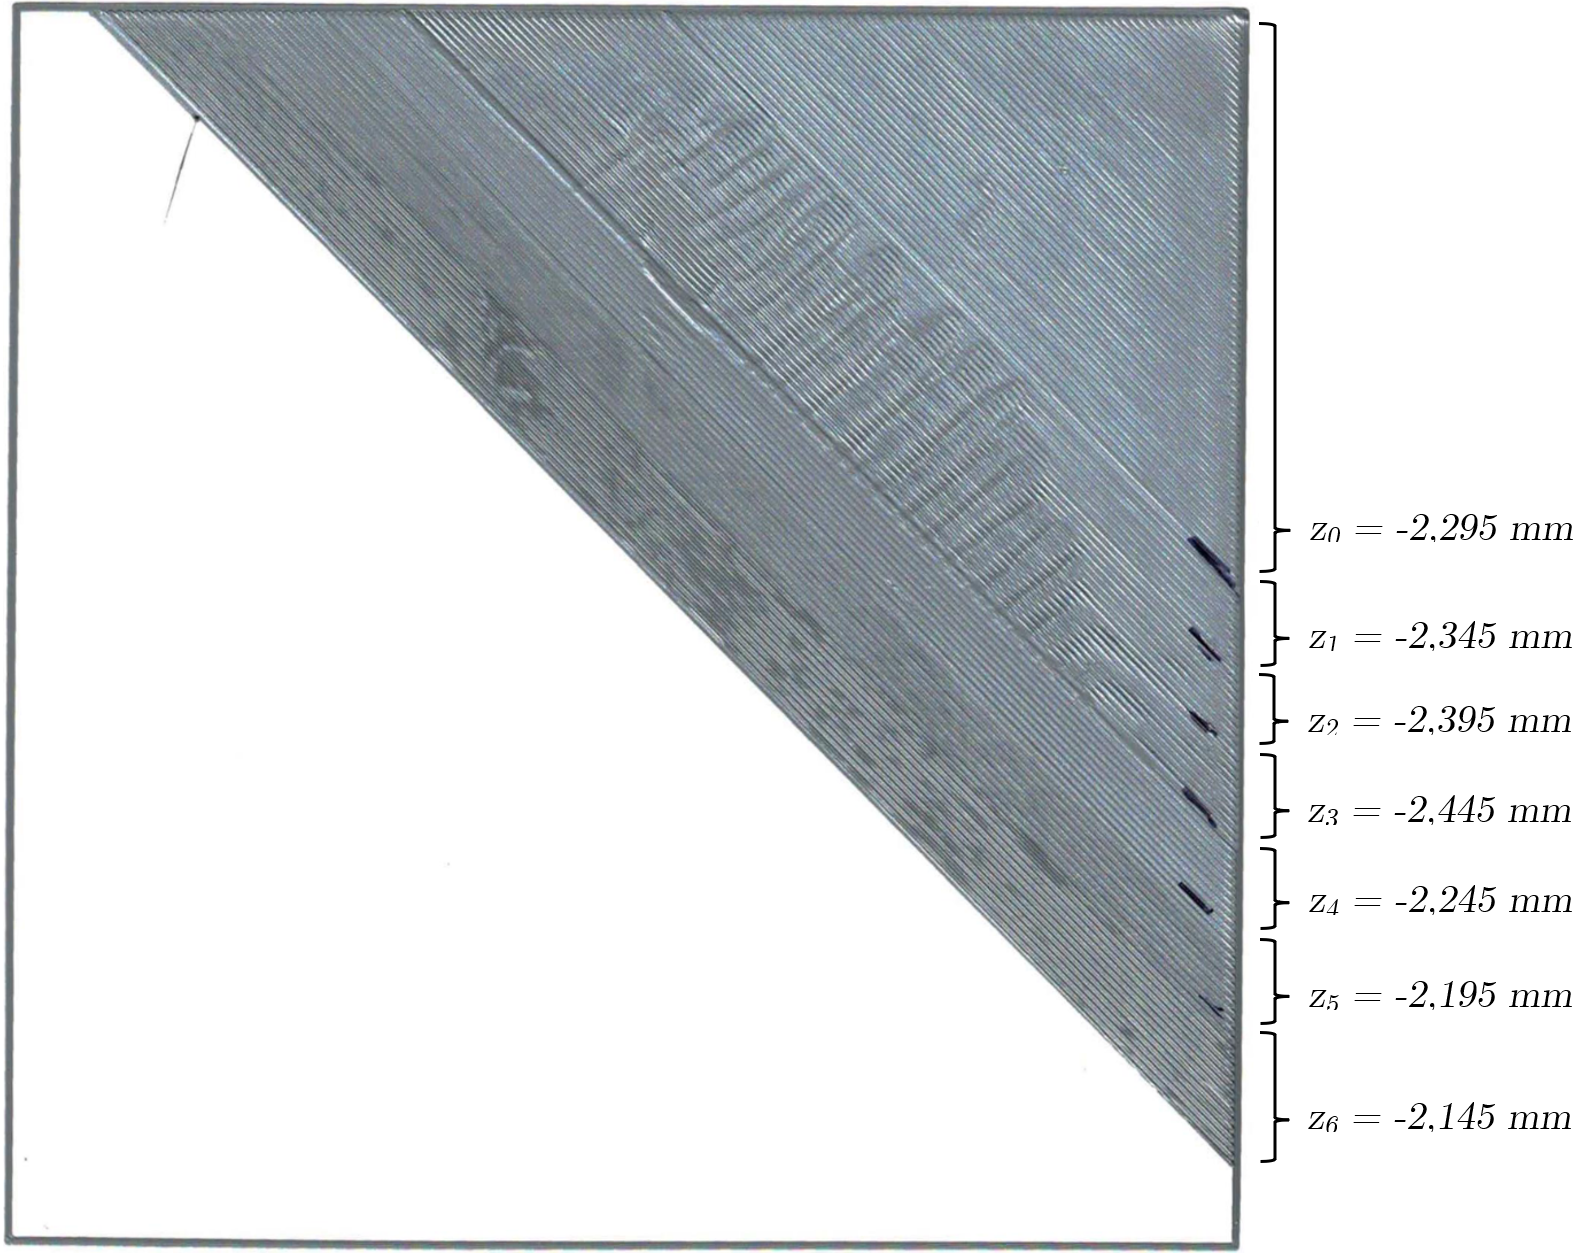
\includegraphics[width=230px]{./images/front.png}}
\caption{Gedrucktes Modell - Oberseite}
\label{front}
\end{figure}

In den Abbilungen \ref*{front} und \ref*{back} ist ein Scan des gedrucken Objektes zu sehen. In den Bereichen von $z_1$ bis $z_3$ befindet sich der Druckkopf dabei näher am Druckbett, was dazu führt, dass das extrudierte Material in der Höhe nicht mehr genug Platz findet und sich daraufhin auch zur Seite hin ausbreitet. Die Folge dessen ist dann, dass die weiteren Fahrten des Druckkopfes vorbei an den zu breit aufgetragenen Schichten selbiges Problem haben, das Material dann aber nur noch in eine Richting ausweichen kann. Das ganze führt zu einer Wellenartigen Struktur, die man besonders in der Sicht von oben in Abbildung \ref*{front} erkennen kann.

Die Folgen eines zu großen Abstandes zu Druckbett lassen sich in Abbildung \ref*{back} besser erkennen, denn schon bei der ersten Erhöhung $z_4$ haftet das Material nicht mehr ideal an der Druckplatte. Bei $z_6$ lassen sich bereits Spalten zwischen den Strängen an Material erkennen, was darauf schließen lässt, dass diese sich nicht miteinander verbinden konnten und so keine geschlossene Schicht entstanden ist. 
\begin{figure}[htbp]
\centerline{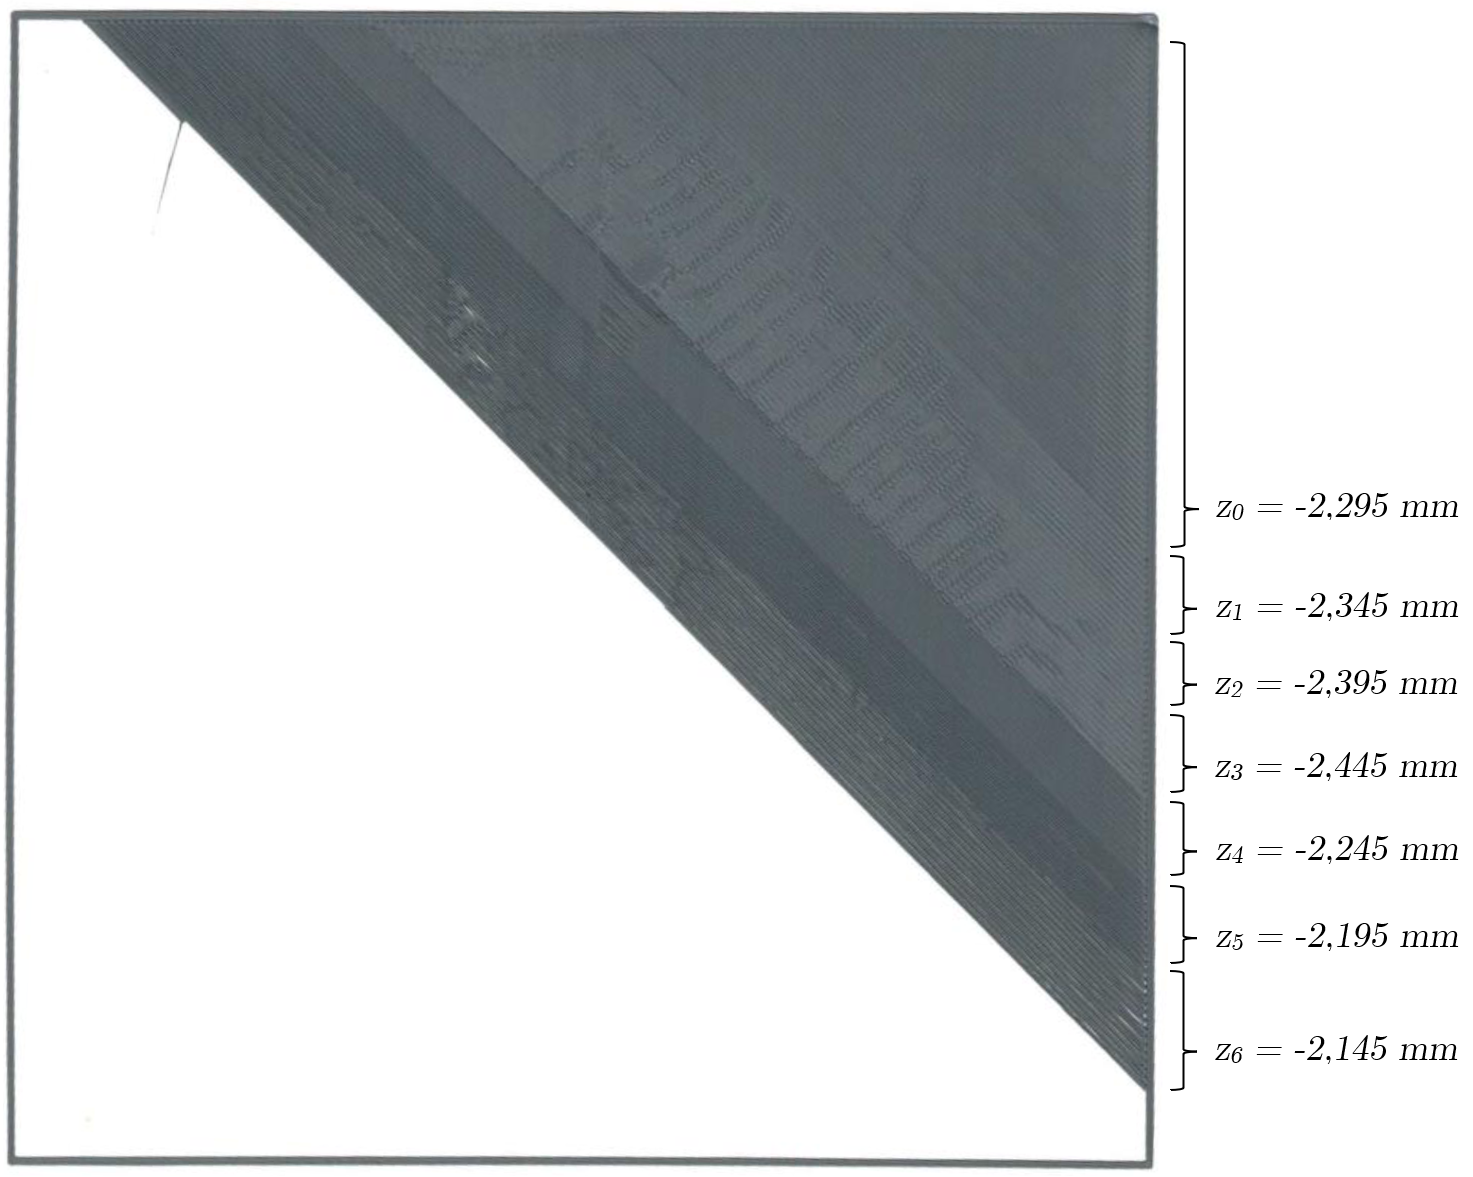
\includegraphics[width=230px]{./images/back.png}}
\caption{Gedrucktes Modell - Unterseite}
\label{back}
\end{figure}

Abschließend lässt sich sagen, dass beide Richtungen der Höhenverstellung zeigten, wie wichtig die Bedeutung der korrekte Höhe des Druckkopfes für einen erfolgreichen Druck ist. Sowohl ein zu nah als auch zu fern eingestellter Kopf führt dazu, dass das Material sich unterienander schlecht verbindet und die Haftung zum Druckbett nicht ideal ist. Diese Haftung ist speziell für den späteren Verlauf eines Druckes wichtig.

%Hier wird eine Quelle zitiert \cite{Quelle}.
\newpage
\begin{thebibliography}{999}
\bibitem{Quelle} Versuchsanleitung zu (Abgerufen am 23.03.2022) 
\end{thebibliography}

% Für Dokumente mit mehr Referenzen empfiehlt es sich, auf eine separate .bib -Datei umzusteigen, die alle Referenzen enthält. Diese Referenzen können bei den meisten wissenschaftlichen Publikationen direkt über "BibTex-Export" oder ähnliches heruntergeladen werden. Anstelle von \begin{thebibliography}...\bibitem{}..\bibitem{}..\end{thebibliography} muss dann lediglich \bibliography{Dateiname.bib} eingebunden werden.

%\section{Anhang}
%\includepdf[pages=-]{Dateiname.pdf}


\end{document}